\documentclass[1p]{elsarticle_modified}
%\bibliographystyle{elsarticle-num}

%\usepackage[colorlinks]{hyperref}
%\usepackage{abbrmath_seonhwa} %\Abb, \Ascr, \Acal ,\Abf, \Afrak
\usepackage{amsfonts}
\usepackage{amssymb}
\usepackage{amsmath}
\usepackage{amsthm}
\usepackage{scalefnt}
\usepackage{amsbsy}
\usepackage{kotex}
\usepackage{caption}
\usepackage{subfig}
\usepackage{color}
\usepackage{graphicx}
\usepackage{xcolor} %% white, black, red, green, blue, cyan, magenta, yellow
\usepackage{float}
\usepackage{setspace}
\usepackage{hyperref}

\usepackage{tikz}
\usetikzlibrary{arrows}

\usepackage{multirow}
\usepackage{array} % fixed length table
\usepackage{hhline}

%%%%%%%%%%%%%%%%%%%%%
\makeatletter
\renewcommand*\env@matrix[1][\arraystretch]{%
	\edef\arraystretch{#1}%
	\hskip -\arraycolsep
	\let\@ifnextchar\new@ifnextchar
	\array{*\c@MaxMatrixCols c}}
\makeatother %https://tex.stackexchange.com/questions/14071/how-can-i-increase-the-line-spacing-in-a-matrix
%%%%%%%%%%%%%%%

\usepackage[normalem]{ulem}

\newcommand{\msout}[1]{\ifmmode\text{\sout{\ensuremath{#1}}}\else\sout{#1}\fi}
%SOURCE: \msout is \stkout macro in https://tex.stackexchange.com/questions/20609/strikeout-in-math-mode

\newcommand{\cancel}[1]{
	\ifmmode
	{\color{red}\msout{#1}}
	\else
	{\color{red}\sout{#1}}
	\fi
}

\newcommand{\add}[1]{
	{\color{blue}\uwave{#1}}
}

\newcommand{\replace}[2]{
	\ifmmode
	{\color{red}\msout{#1}}{\color{blue}\uwave{#2}}
	\else
	{\color{red}\sout{#1}}{\color{blue}\uwave{#2}}
	\fi
}

\newcommand{\Sol}{\mathcal{S}} %segment
\newcommand{\D}{D} %diagram
\newcommand{\A}{\mathcal{A}} %arc


%%%%%%%%%%%%%%%%%%%%%%%%%%%%%5 test

\def\sl{\operatorname{\textup{SL}}(2,\Cbb)}
\def\psl{\operatorname{\textup{PSL}}(2,\Cbb)}
\def\quan{\mkern 1mu \triangleright \mkern 1mu}

\theoremstyle{definition}
\newtheorem{thm}{Theorem}[section]
\newtheorem{prop}[thm]{Proposition}
\newtheorem{lem}[thm]{Lemma}
\newtheorem{ques}[thm]{Question}
\newtheorem{cor}[thm]{Corollary}
\newtheorem{defn}[thm]{Definition}
\newtheorem{exam}[thm]{Example}
\newtheorem{rmk}[thm]{Remark}
\newtheorem{alg}[thm]{Algorithm}

\newcommand{\I}{\sqrt{-1}}
\begin{document}

%\begin{frontmatter}
%
%\title{Boundary parabolic representations of knots up to 8 crossings}
%
%%% Group authors per affiliation:
%\author{Yunhi Cho} 
%\address{Department of Mathematics, University of Seoul, Seoul, Korea}
%\ead{yhcho@uos.ac.kr}
%
%
%\author{Seonhwa Kim} %\fnref{s_kim}}
%\address{Center for Geometry and Physics, Institute for Basic Science, Pohang, 37673, Korea}
%\ead{ryeona17@ibs.re.kr}
%
%\author{Hyuk Kim}
%\address{Department of Mathematical Sciences, Seoul National University, Seoul 08826, Korea}
%\ead{hyukkim@snu.ac.kr}
%
%\author{Seokbeom Yoon}
%\address{Department of Mathematical Sciences, Seoul National University, Seoul, 08826,  Korea}
%\ead{sbyoon15@snu.ac.kr}
%
%\begin{abstract}
%We find all boundary parabolic representation of knots up to 8 crossings.
%
%\end{abstract}
%\begin{keyword}
%    \MSC[2010] 57M25 
%\end{keyword}
%
%\end{frontmatter}

%\linenumbers
%\tableofcontents
%
\newcommand\colored[1]{\textcolor{white}{\rule[-0.35ex]{0.8em}{1.4ex}}\kern-0.8em\color{red} #1}%
%\newcommand\colored[1]{\textcolor{white}{ #1}\kern-2.17ex	\textcolor{white}{ #1}\kern-1.81ex	\textcolor{white}{ #1}\kern-2.15ex\color{red}#1	}

{\Large $\underline{10_{30}~(K10a_{34})}$}

\setlength{\tabcolsep}{10pt}
\renewcommand{\arraystretch}{1.6}
\vspace{1cm}\begin{tabular}{m{100pt}>{\centering\arraybackslash}m{274pt}}
\multirow{5}{120pt}{
	\centering
	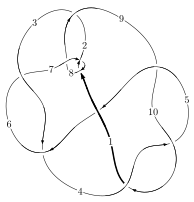
\includegraphics[width=112pt]{../../../GIT/diagram.site/Diagrams/png/114_10_30.png}\\
\ \ \ A knot diagram\footnotemark}&
\allowdisplaybreaks
\textbf{Linearized knot diagam} \\
\cline{2-2}
 &
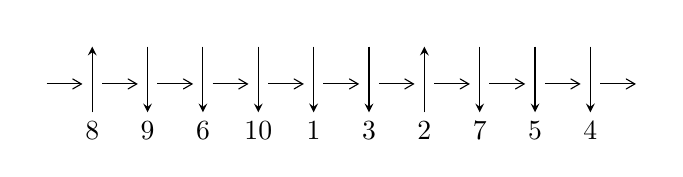
\begin{tikzpicture}[x=20pt, y=17pt]
	% nodes
	\node (C0) at (0, 0) {};
	\node (C1) at (1, 0) {};
	\node (C1U) at (1, +1) {};
	\node (C1D) at (1, -1) {8};

	\node (C2) at (2, 0) {};
	\node (C2U) at (2, +1) {};
	\node (C2D) at (2, -1) {9};

	\node (C3) at (3, 0) {};
	\node (C3U) at (3, +1) {};
	\node (C3D) at (3, -1) {6};

	\node (C4) at (4, 0) {};
	\node (C4U) at (4, +1) {};
	\node (C4D) at (4, -1) {10};

	\node (C5) at (5, 0) {};
	\node (C5U) at (5, +1) {};
	\node (C5D) at (5, -1) {1};

	\node (C6) at (6, 0) {};
	\node (C6U) at (6, +1) {};
	\node (C6D) at (6, -1) {3};

	\node (C7) at (7, 0) {};
	\node (C7U) at (7, +1) {};
	\node (C7D) at (7, -1) {2};

	\node (C8) at (8, 0) {};
	\node (C8U) at (8, +1) {};
	\node (C8D) at (8, -1) {7};

	\node (C9) at (9, 0) {};
	\node (C9U) at (9, +1) {};
	\node (C9D) at (9, -1) {5};

	\node (C10) at (10, 0) {};
	\node (C10U) at (10, +1) {};
	\node (C10D) at (10, -1) {4};
	\node (C11) at (11, 0) {};

	% arrows
	\draw[->,>={angle 60}]
	(C0) edge (C1) (C1) edge (C2) (C2) edge (C3) (C3) edge (C4) (C4) edge (C5) (C5) edge (C6) (C6) edge (C7) (C7) edge (C8) (C8) edge (C9) (C9) edge (C10) (C10) edge (C11) ;	\draw[->,>=stealth]
	(C1D) edge (C1U) (C2U) edge (C2D) (C3U) edge (C3D) (C4U) edge (C4D) (C5U) edge (C5D) (C6U) edge (C6D) (C7D) edge (C7U) (C8U) edge (C8D) (C9U) edge (C9D) (C10U) edge (C10D) ;
	\end{tikzpicture} \\
\hhline{~~} \\& 
\textbf{Solving Sequence} \\ \cline{2-2} 
 &
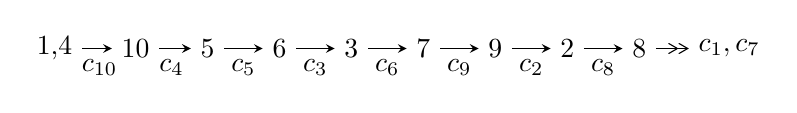
\begin{tikzpicture}[x=26pt, y=7pt]
	% node
	\node (A0) at (-1/8, 0) {1,4};
	\node (A1) at (1, 0) {10};
	\node (A2) at (2, 0) {5};
	\node (A3) at (3, 0) {6};
	\node (A4) at (4, 0) {3};
	\node (A5) at (5, 0) {7};
	\node (A6) at (6, 0) {9};
	\node (A7) at (7, 0) {2};
	\node (A8) at (8, 0) {8};
	\node (C1) at (1/2, -1) {$c_{10}$};
	\node (C2) at (3/2, -1) {$c_{4}$};
	\node (C3) at (5/2, -1) {$c_{5}$};
	\node (C4) at (7/2, -1) {$c_{3}$};
	\node (C5) at (9/2, -1) {$c_{6}$};
	\node (C6) at (11/2, -1) {$c_{9}$};
	\node (C7) at (13/2, -1) {$c_{2}$};
	\node (C8) at (15/2, -1) {$c_{8}$};
	\node (A9) at (37/4, 0) {$c_{1},c_{7}$};

	% edge
	\draw[->,>=stealth]	
	(A0) edge (A1) (A1) edge (A2) (A2) edge (A3) (A3) edge (A4) (A4) edge (A5) (A5) edge (A6) (A6) edge (A7) (A7) edge (A8) ;
	\draw[->>,>={angle 60}]	
	(A8) edge (A9);
\end{tikzpicture} \\ 

\end{tabular} \\

\footnotetext{
The image of knot diagram is generated by the software ``\textbf{Draw programme}" developed by Andrew Bartholomew(\url{http://www.layer8.co.uk/maths/draw/index.htm\#Running-draw}), where we modified some parts for our purpose(\url{https://github.com/CATsTAILs/LinksPainter}).
}\phantom \\ \newline 
\centering \textbf{Ideals for irreducible components\footnotemark of $X_{\text{par}}$} 
 
\begin{align*}
I^u_{1}&=\langle 
u^{33}- u^{32}+\cdots+3 u-1\rangle \\
\\
\end{align*}
\raggedright * 1 irreducible components of $\dim_{\mathbb{C}}=0$, with total 33 representations.\\
\footnotetext{All coefficients of polynomials are rational numbers. But the coefficients are sometimes approximated in decimal forms when there is not enough margin.}
\newpage
\renewcommand{\arraystretch}{1}
\centering \section*{I. $I^u_{1}= \langle u^{33}- u^{32}+\cdots+3 u-1 \rangle$}
\flushleft \textbf{(i) Arc colorings}\\
\begin{tabular}{m{7pt} m{180pt} m{7pt} m{180pt} }
\flushright $a_{1}=$&$\begin{pmatrix}1\\0\end{pmatrix}$ \\
\flushright $a_{4}=$&$\begin{pmatrix}0\\u\end{pmatrix}$ \\
\flushright $a_{10}=$&$\begin{pmatrix}1\\- u^2\end{pmatrix}$ \\
\flushright $a_{5}=$&$\begin{pmatrix}- u\\u^3+u\end{pmatrix}$ \\
\flushright $a_{6}=$&$\begin{pmatrix}- u^3-2 u\\u^3+u\end{pmatrix}$ \\
\flushright $a_{3}=$&$\begin{pmatrix}u^7+4 u^5+4 u^3\\- u^7-3 u^5-2 u^3+u\end{pmatrix}$ \\
\flushright $a_{7}=$&$\begin{pmatrix}- u^{11}-6 u^9-12 u^7-8 u^5- u^3-2 u\\u^{11}+5 u^9+8 u^7+3 u^5- u^3+u\end{pmatrix}$ \\
\flushright $a_{9}=$&$\begin{pmatrix}u^2+1\\- u^4-2 u^2\end{pmatrix}$ \\
\flushright $a_{2}=$&$\begin{pmatrix}u^{13}+6 u^{11}+13 u^9+12 u^7+6 u^5+4 u^3+u\\- u^{15}-7 u^{13}-18 u^{11}-19 u^9-6 u^7-2 u^5-4 u^3+u\end{pmatrix}$ \\
\flushright $a_{8}=$&$\begin{pmatrix}- u^{26}-13 u^{24}+\cdots+3 u^2+1\\u^{26}+12 u^{24}+\cdots+4 u^4-3 u^2\end{pmatrix}$\\&\end{tabular}
\flushleft \textbf{(ii) Obstruction class $= -1$}\\~\\
\flushleft \textbf{(iii) Cusp Shapes $= -4 u^{32}+4 u^{31}-64 u^{30}+56 u^{29}-448 u^{28}+340 u^{27}-1788 u^{26}+1156 u^{25}-4432 u^{24}+2356 u^{23}-6940 u^{22}+2804 u^{21}-6652 u^{20}+1616 u^{19}-3660 u^{18}+8 u^{17}-1380 u^{16}-364 u^{15}-932 u^{14}-156 u^{13}-380 u^{12}-360 u^{11}+224 u^{10}-328 u^9+40 u^8-4 u^7-56 u^6+4 u^5+48 u^4-32 u^3-12 u^2+20 u-14$}\\~\\
\newpage\renewcommand{\arraystretch}{1}
\flushleft \textbf{(iv) u-Polynomials at the component}\newline \\
\begin{tabular}{m{50pt}|m{274pt}}
Crossings & \hspace{64pt}u-Polynomials at each crossing \\
\hline $$\begin{aligned}c_{1},c_{7}\end{aligned}$$&$\begin{aligned}
&u^{33}- u^{32}+\cdots- u+1
\end{aligned}$\\
\hline $$\begin{aligned}c_{2}\end{aligned}$$&$\begin{aligned}
&u^{33}+u^{32}+\cdots+u+1
\end{aligned}$\\
\hline $$\begin{aligned}c_{3},c_{6}\end{aligned}$$&$\begin{aligned}
&u^{33}-5 u^{32}+\cdots-31 u+3
\end{aligned}$\\
\hline $$\begin{aligned}c_{4},c_{9},c_{10}\end{aligned}$$&$\begin{aligned}
&u^{33}+u^{32}+\cdots+3 u+1
\end{aligned}$\\
\hline $$\begin{aligned}c_{5}\end{aligned}$$&$\begin{aligned}
&u^{33}- u^{32}+\cdots+61 u+17
\end{aligned}$\\
\hline $$\begin{aligned}c_{8}\end{aligned}$$&$\begin{aligned}
&u^{33}+15 u^{32}+\cdots+u-1
\end{aligned}$\\
\hline
\end{tabular}\\~\\
\newpage\renewcommand{\arraystretch}{1}
\flushleft \textbf{(v) Riley Polynomials at the component}\newline \\
\begin{tabular}{m{50pt}|m{274pt}}
Crossings & \hspace{64pt}Riley Polynomials at each crossing \\
\hline $$\begin{aligned}c_{1},c_{7}\end{aligned}$$&$\begin{aligned}
&y^{33}+15 y^{32}+\cdots+y-1
\end{aligned}$\\
\hline $$\begin{aligned}c_{2}\end{aligned}$$&$\begin{aligned}
&y^{33}- y^{32}+\cdots+33 y-1
\end{aligned}$\\
\hline $$\begin{aligned}c_{3},c_{6}\end{aligned}$$&$\begin{aligned}
&y^{33}+27 y^{32}+\cdots+y-9
\end{aligned}$\\
\hline $$\begin{aligned}c_{4},c_{9},c_{10}\end{aligned}$$&$\begin{aligned}
&y^{33}+31 y^{32}+\cdots+y-1
\end{aligned}$\\
\hline $$\begin{aligned}c_{5}\end{aligned}$$&$\begin{aligned}
&y^{33}+11 y^{32}+\cdots-3011 y-289
\end{aligned}$\\
\hline $$\begin{aligned}c_{8}\end{aligned}$$&$\begin{aligned}
&y^{33}+7 y^{32}+\cdots+17 y-1
\end{aligned}$\\
\hline
\end{tabular}\\~\\
\newpage\flushleft \textbf{(vi) Complex Volumes and Cusp Shapes}
$$\begin{array}{c|c|c}  
\text{Solutions to }I^u_{1}& \I (\text{vol} + \sqrt{-1}CS) & \text{Cusp shape}\\
 \hline 
\begin{aligned}
u &= -0.138722 + 1.178260 I\end{aligned}
 & -0.390154 - 0.572456 I & -8.31906 + 0.48605 I \\ \hline\begin{aligned}
u &= -0.138722 - 1.178260 I\end{aligned}
 & -0.390154 + 0.572456 I & -8.31906 - 0.48605 I \\ \hline\begin{aligned}
u &= \phantom{-}0.679432 + 0.391507 I\end{aligned}
 & \phantom{-}1.46905 - 8.41845 I & -5.65597 + 8.08731 I \\ \hline\begin{aligned}
u &= \phantom{-}0.679432 - 0.391507 I\end{aligned}
 & \phantom{-}1.46905 + 8.41845 I & -5.65597 - 8.08731 I \\ \hline\begin{aligned}
u &= -0.649750 + 0.407780 I\end{aligned}
 & \phantom{-}3.38108 + 3.30675 I & -2.44424 - 3.71770 I \\ \hline\begin{aligned}
u &= -0.649750 - 0.407780 I\end{aligned}
 & \phantom{-}3.38108 - 3.30675 I & -2.44424 + 3.71770 I \\ \hline\begin{aligned}
u &= \phantom{-}0.552937 + 0.519363 I\end{aligned}
 & \phantom{-}1.99857 + 4.30723 I & -4.15179 - 2.03529 I \\ \hline\begin{aligned}
u &= \phantom{-}0.552937 - 0.519363 I\end{aligned}
 & \phantom{-}1.99857 - 4.30723 I & -4.15179 + 2.03529 I \\ \hline\begin{aligned}
u &= -0.578988 + 0.474023 I\end{aligned}
 & \phantom{-}3.67259 + 0.72831 I & -1.49015 - 3.12560 I \\ \hline\begin{aligned}
u &= -0.578988 - 0.474023 I\end{aligned}
 & \phantom{-}3.67259 - 0.72831 I & -1.49015 + 3.12560 I \\ \hline\begin{aligned}
u &= -0.214004 + 1.270020 I\end{aligned}
 & \phantom{-}0.50606 + 6.56196 I & -6.35976 - 7.19745 I \\ \hline\begin{aligned}
u &= -0.214004 - 1.270020 I\end{aligned}
 & \phantom{-}0.50606 - 6.56196 I & -6.35976 + 7.19745 I \\ \hline\begin{aligned}
u &= \phantom{-}0.150986 + 1.283520 I\end{aligned}
 & \phantom{-}2.96939 - 2.39560 I & -2.36922 + 3.31266 I \\ \hline\begin{aligned}
u &= \phantom{-}0.150986 - 1.283520 I\end{aligned}
 & \phantom{-}2.96939 + 2.39560 I & -2.36922 - 3.31266 I \\ \hline\begin{aligned}
u &= \phantom{-}0.596688 + 0.315979 I\end{aligned}
 & -1.43040 - 1.50384 I & -9.59059 + 3.60616 I \\ \hline\begin{aligned}
u &= \phantom{-}0.596688 - 0.315979 I\end{aligned}
 & -1.43040 + 1.50384 I & -9.59059 - 3.60616 I \\ \hline\begin{aligned}
u &= -0.632184 + 0.066503 I\end{aligned}
 & -3.60742 + 3.47782 I & -12.61515 - 4.95314 I \\ \hline\begin{aligned}
u &= -0.632184 - 0.066503 I\end{aligned}
 & -3.60742 - 3.47782 I & -12.61515 + 4.95314 I \\ \hline\begin{aligned}
u &= \phantom{-}0.036115 + 1.379920 I\end{aligned}
 & \phantom{-}4.95997 - 2.19825 I & \phantom{-}0.55384 + 3.61625 I \\ \hline\begin{aligned}
u &= \phantom{-}0.036115 - 1.379920 I\end{aligned}
 & \phantom{-}4.95997 + 2.19825 I & \phantom{-}0.55384 - 3.61625 I \\ \hline\begin{aligned}
u &= \phantom{-}0.22801 + 1.42935 I\end{aligned}
 & \phantom{-}4.19152 - 4.53523 I & -6.00000 + 3.09222 I \\ \hline\begin{aligned}
u &= \phantom{-}0.22801 - 1.42935 I\end{aligned}
 & \phantom{-}4.19152 + 4.53523 I & -6.00000 - 3.09222 I \\ \hline\begin{aligned}
u &= -0.24113 + 1.46019 I\end{aligned}
 & \phantom{-}9.39642 + 6.56751 I & \phantom{-0.000000 } 0. - 3.41838 I \\ \hline\begin{aligned}
u &= -0.24113 - 1.46019 I\end{aligned}
 & \phantom{-}9.39642 - 6.56751 I & \phantom{-0.000000 -}0. + 3.41838 I \\ \hline\begin{aligned}
u &= \phantom{-}0.25408 + 1.45840 I\end{aligned}
 & \phantom{-}7.42465 - 11.82880 I & \phantom{-0.000000 -}0. + 7.75337 I \\ \hline\begin{aligned}
u &= \phantom{-}0.25408 - 1.45840 I\end{aligned}
 & \phantom{-}7.42465 + 11.82880 I & \phantom{-0.000000 } 0. - 7.75337 I \\ \hline\begin{aligned}
u &= -0.20598 + 1.46844 I\end{aligned}
 & \phantom{-}9.92249 + 3.59396 I & \phantom{-0.000000 } 0. - 3.03909 I \\ \hline\begin{aligned}
u &= -0.20598 - 1.46844 I\end{aligned}
 & \phantom{-}9.92249 - 3.59396 I & \phantom{-0.000000 -}0. + 3.03909 I \\ \hline\begin{aligned}
u &= \phantom{-}0.18821 + 1.47294 I\end{aligned}
 & \phantom{-}8.40124 + 1.63491 I & \phantom{-0.000000 } 0 \\ \hline\begin{aligned}
u &= \phantom{-}0.18821 - 1.47294 I\end{aligned}
 & \phantom{-}8.40124 - 1.63491 I & \phantom{-0.000000 } 0\\
 \hline 
 \end{array}$$\newpage$$\begin{array}{c|c|c}  
\text{Solutions to }I^u_{1}& \I (\text{vol} + \sqrt{-1}CS) & \text{Cusp shape}\\
 \hline 
\begin{aligned}
u &= \phantom{-}0.514867\phantom{ +0.000000I}\end{aligned}
 & -1.00604\phantom{ +0.000000I} & -9.72740\phantom{ +0.000000I} \\ \hline\begin{aligned}
u &= \phantom{-}0.216864 + 0.450093 I\end{aligned}
 & -0.54661 - 1.45331 I & -5.02647 + 4.36257 I \\ \hline\begin{aligned}
u &= \phantom{-}0.216864 - 0.450093 I\end{aligned}
 & -0.54661 + 1.45331 I & -5.02647 - 4.36257 I\\
 \hline 
 \end{array}$$\newpage
\newpage\renewcommand{\arraystretch}{1}
\centering \section*{ II. u-Polynomials}
\begin{tabular}{m{50pt}|m{274pt}}
Crossings & \hspace{64pt}u-Polynomials at each crossing \\
\hline $$\begin{aligned}c_{1},c_{7}\end{aligned}$$&$\begin{aligned}
&u^{33}- u^{32}+\cdots- u+1
\end{aligned}$\\
\hline $$\begin{aligned}c_{2}\end{aligned}$$&$\begin{aligned}
&u^{33}+u^{32}+\cdots+u+1
\end{aligned}$\\
\hline $$\begin{aligned}c_{3},c_{6}\end{aligned}$$&$\begin{aligned}
&u^{33}-5 u^{32}+\cdots-31 u+3
\end{aligned}$\\
\hline $$\begin{aligned}c_{4},c_{9},c_{10}\end{aligned}$$&$\begin{aligned}
&u^{33}+u^{32}+\cdots+3 u+1
\end{aligned}$\\
\hline $$\begin{aligned}c_{5}\end{aligned}$$&$\begin{aligned}
&u^{33}- u^{32}+\cdots+61 u+17
\end{aligned}$\\
\hline $$\begin{aligned}c_{8}\end{aligned}$$&$\begin{aligned}
&u^{33}+15 u^{32}+\cdots+u-1
\end{aligned}$\\
\hline
\end{tabular}\newpage\renewcommand{\arraystretch}{1}
\centering \section*{ III. Riley Polynomials}
\begin{tabular}{m{50pt}|m{274pt}}
Crossings & \hspace{64pt}Riley Polynomials at each crossing \\
\hline $$\begin{aligned}c_{1},c_{7}\end{aligned}$$&$\begin{aligned}
&y^{33}+15 y^{32}+\cdots+y-1
\end{aligned}$\\
\hline $$\begin{aligned}c_{2}\end{aligned}$$&$\begin{aligned}
&y^{33}- y^{32}+\cdots+33 y-1
\end{aligned}$\\
\hline $$\begin{aligned}c_{3},c_{6}\end{aligned}$$&$\begin{aligned}
&y^{33}+27 y^{32}+\cdots+y-9
\end{aligned}$\\
\hline $$\begin{aligned}c_{4},c_{9},c_{10}\end{aligned}$$&$\begin{aligned}
&y^{33}+31 y^{32}+\cdots+y-1
\end{aligned}$\\
\hline $$\begin{aligned}c_{5}\end{aligned}$$&$\begin{aligned}
&y^{33}+11 y^{32}+\cdots-3011 y-289
\end{aligned}$\\
\hline $$\begin{aligned}c_{8}\end{aligned}$$&$\begin{aligned}
&y^{33}+7 y^{32}+\cdots+17 y-1
\end{aligned}$\\
\hline
\end{tabular}
\vskip 2pc
\end{document}